\documentclass[pdftex,12pt,a4paper]{article}

\usepackage{graphicx}  
\usepackage[margin=2.5cm]{geometry}
\usepackage{breakcites}
\usepackage{indentfirst}
\usepackage{pgfgantt}
\usepackage{pdflscape}
\usepackage{float}
\usepackage{epsfig}
\usepackage{epstopdf}
\usepackage[cmex10]{amsmath}
\usepackage{stfloats}
\usepackage{multirow}

\renewcommand{\refname}{REFERENCES}
\linespread{1.3}

\usepackage{mathtools}
%\newcommand{\HRule}{\rule{\linewidth}{0.5mm}}
\thispagestyle{empty}
\begin{document}
\begin{titlepage}
\begin{center}
\textbf{}\\
\textbf{\Large{ISTANBUL TECHNICAL UNIVERSITY}}\\
\vspace{0.5cm}
\textbf{\Large{COMPUTER ENGINEERING DEPARTMENT}}\\
\vspace{2cm}
\textbf{\Large{BLG 242E\\ DIGITAL CIRCUITS LABORATORY\\ EXPERIMENT REPORT}}\\
\vspace{2.8cm}
\begin{table}[ht]
\centering
\Large{
\begin{tabular}{lcl}
\textbf{EXPERIMENT NO}  & : & 1 \\
\textbf{EXPERIMENT DATE}  & : & 14.02.2020 \\
\textbf{LAB SESSION}  & : & FRIDAY - 08.30 \\
\textbf{GROUP NO}  & : & G6 \\
\end{tabular}}
\end{table}
\vspace{1cm}
\textbf{\Large{GROUP MEMBERS:}}\\
\begin{table}[ht]
\centering
\Large{
\begin{tabular}{rcl}
150170087  & : & Sırrı Batuhan ÇOKSAK \\
150170039  & : & Fatih MURAT \\
150160520  & : & Fatih Furkan KAVASOĞLU \\
\end{tabular}}
\end{table}
\vspace{2.8cm}
\textbf{\Large{SPRING 2020}}

\end{center}
\end{titlepage}

\thispagestyle{empty}
\addtocontents{toc}{\contentsline {section}{\numberline {}FRONT COVER}{}}
\addtocontents{toc}{\contentsline {section}{\numberline {}CONTENTS}{}}
\setcounter{tocdepth}{4}
\tableofcontents
\clearpage

\setcounter{page}{1}

\section{INTRODUCTION}

In this experiment we were expected to learn how to work with lab equipment that will be used in future experiments, these lab equipment include multi-meter, function generator, oscilloscope , ICs and CADET components such as breadboard, logic switches, SPDT switches, power supply, potentiometers, logic monitors and displays.

\section{MATERIALS AND EXPERIMENT}

\subsection{PART 1}
In the first part of the experiment we used power supply to generate potential difference of 5 volts, additionally we used breadboard to transfer the potential difference and used multi-meter to measure the potential difference.

\begin{figure}[h]
	\centering
	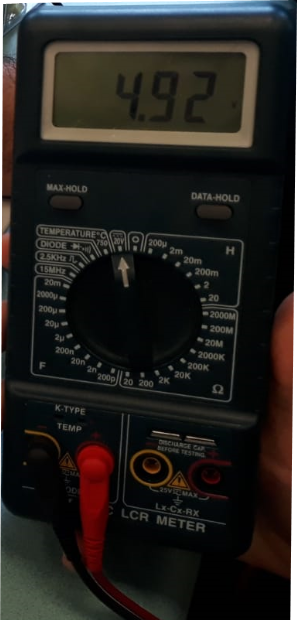
\includegraphics[height=0.5\textwidth]{1.jpg}
	\caption
	\label{Figure 1}
\end{figure}

From the figure 1 we can see that the potential difference is approximately 5 volts 

\clearpage
\subsection{PART 2}
In the second part of the experiment we used an hex inverter IC (7404) to invert the input signal. Initially we used a logic switch to generate the input signal and we connected the output of the IC to the logic monitor to observe the output signal. Secondly we used an SPDT switch instead of logic switch with the power generator and did the same procedure.

\begin{figure}[h]
	\centering
	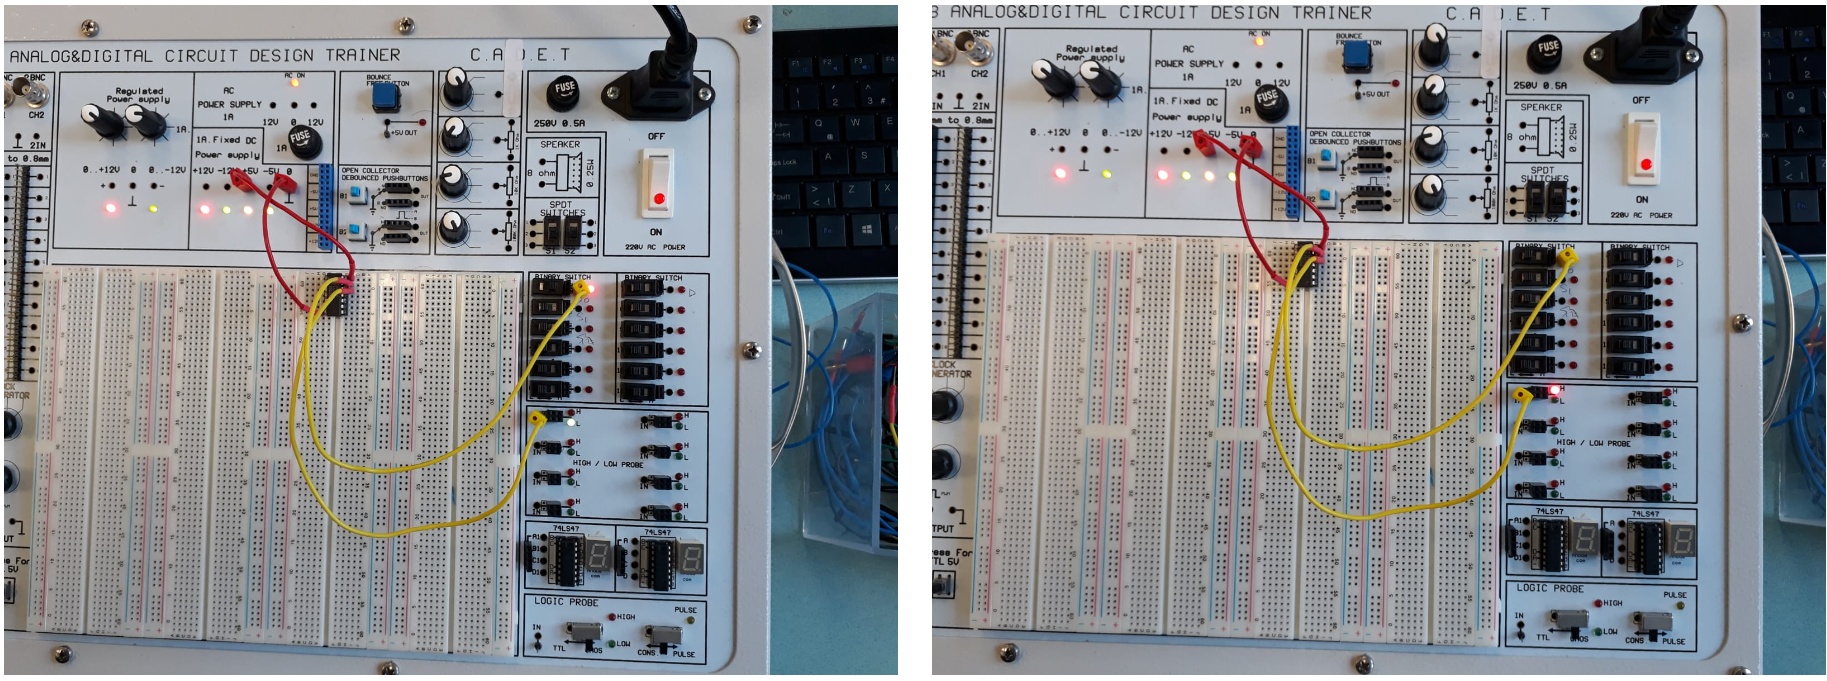
\includegraphics[width=1\textwidth]{2.png}
	\caption
	\label{Figure 2}
\end{figure}

\begin{figure}[h]
	\centering
	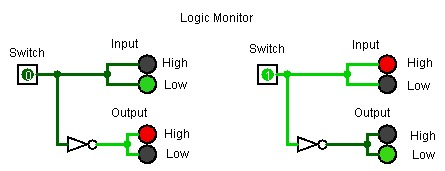
\includegraphics[width=1\textwidth]{3.jpg}
	\caption
	\label{Figure 3}
\end{figure}
From figure 2 and 3, it can be observed that when the input signal is high the output signal is low and when the input signal is low the output signal is high.

\clearpage
\begin{figure}[h]
	\centering
	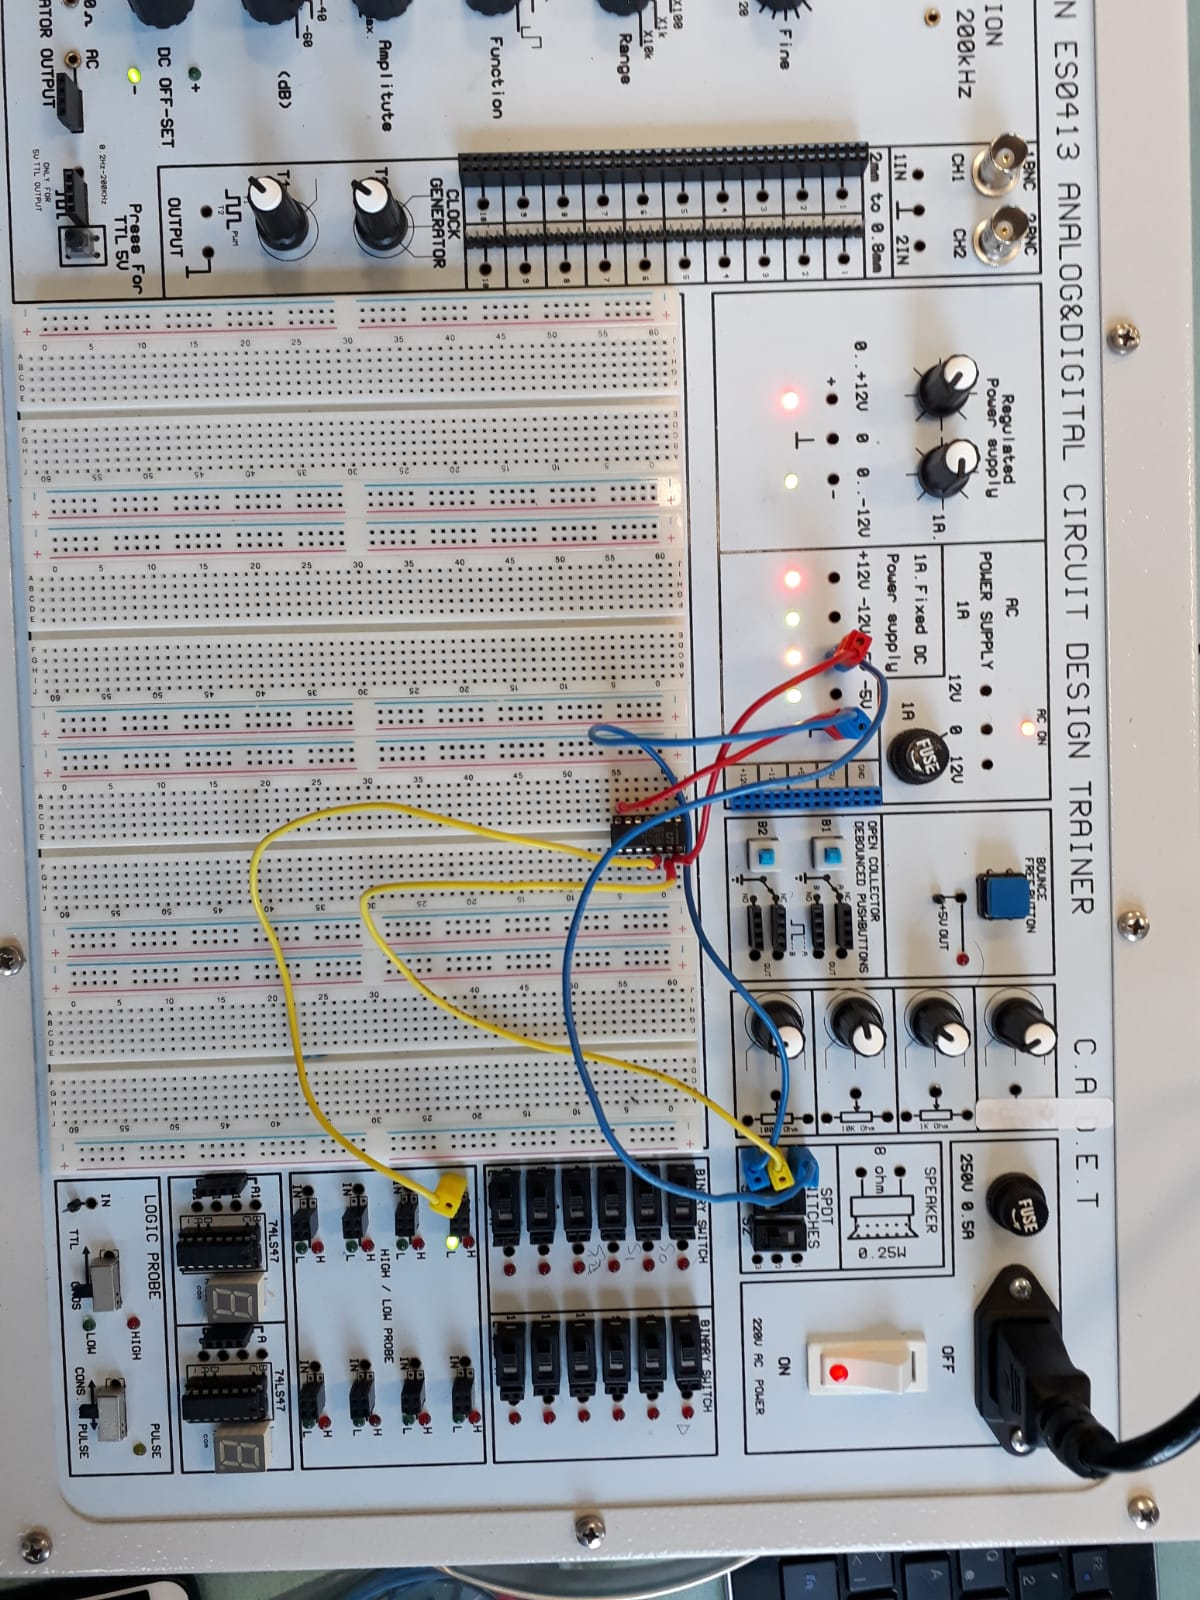
\includegraphics[width=0.5\textwidth, angle = 90 ]{4.jpg}
	\caption
	\label{Figure 4}
\end{figure}

\begin{figure}[h]
    \centering
	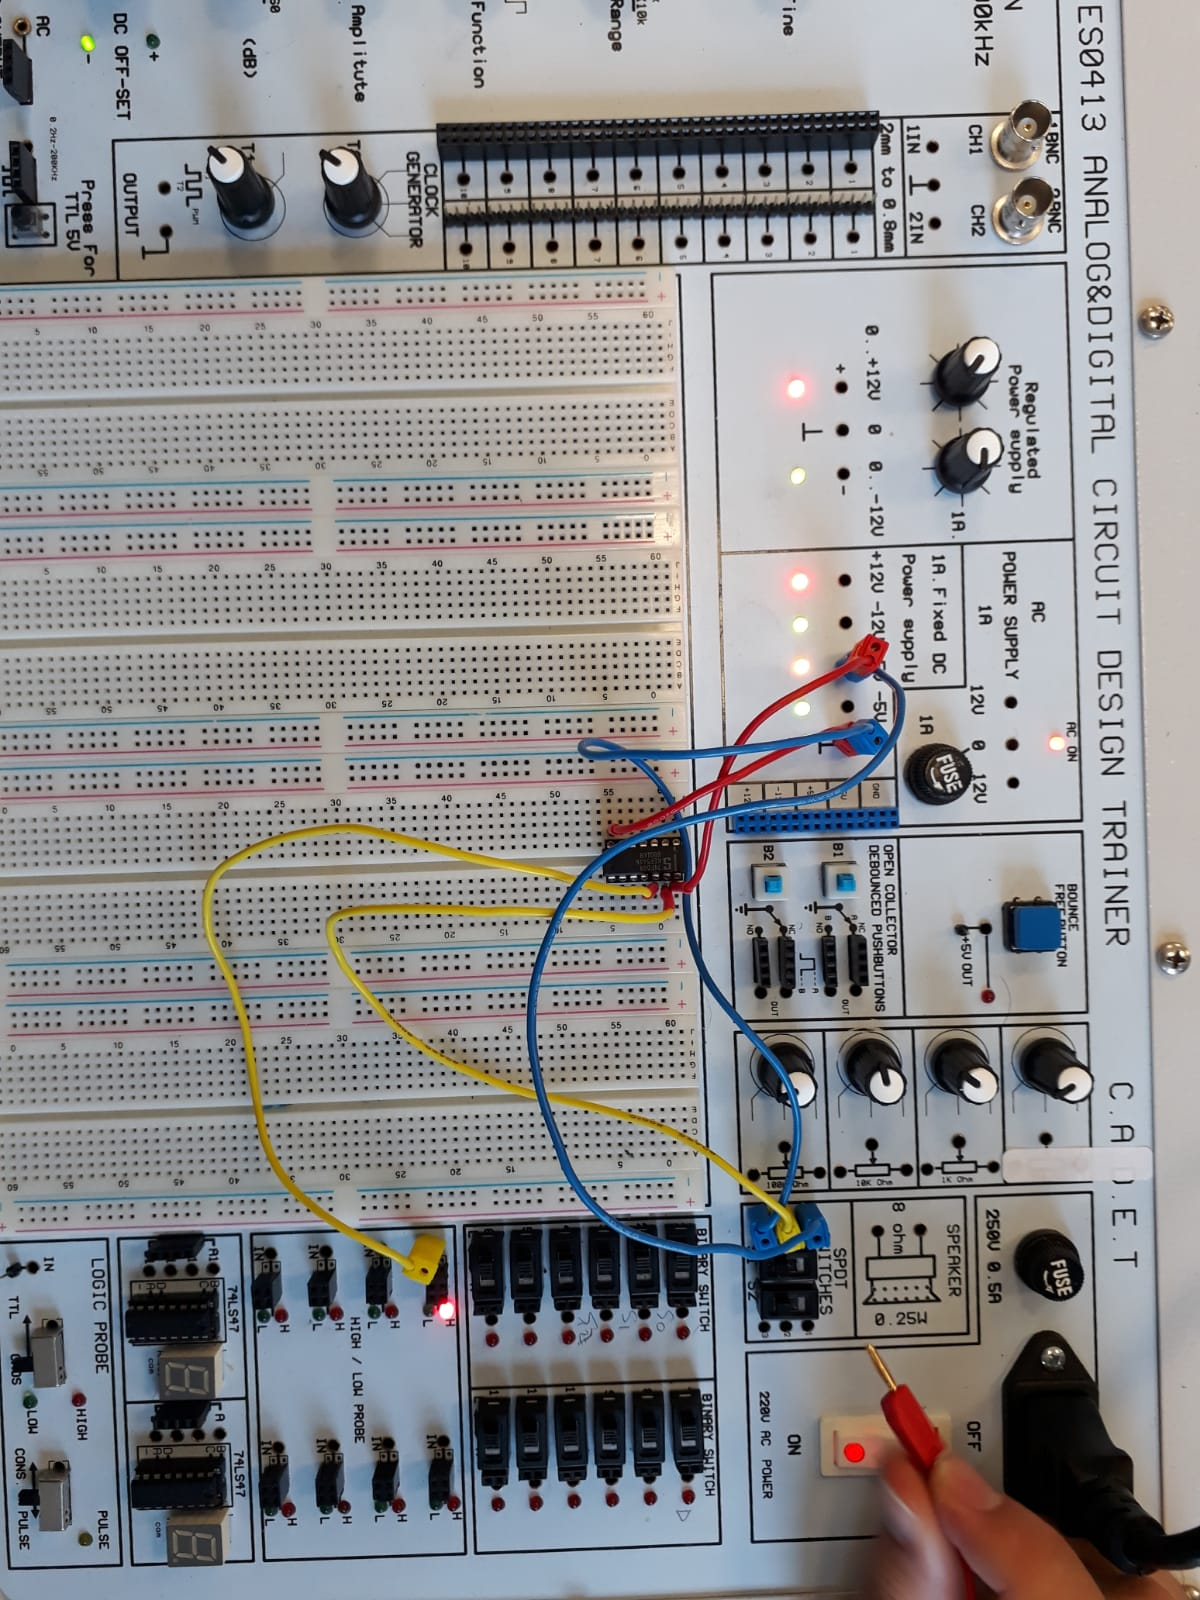
\includegraphics[width=0.5\textwidth, angle = 90 ]{5.jpg}
	\caption
	\label{Figure 5}
\end{figure}

From figure 4 and 5, it is clear that the SPDT switch can be used to switch between two input signals which were set to high and low signals.

\clearpage
\subsection{PART 3}
In this part of the experiment we used power supply to generate potential difference and used voltmeter to measure it, and used potentiometer to obtain resistance of 8 Kohms and used multi-meters resistance measure feature to measure it.

\begin{figure}[h]
	\centering
	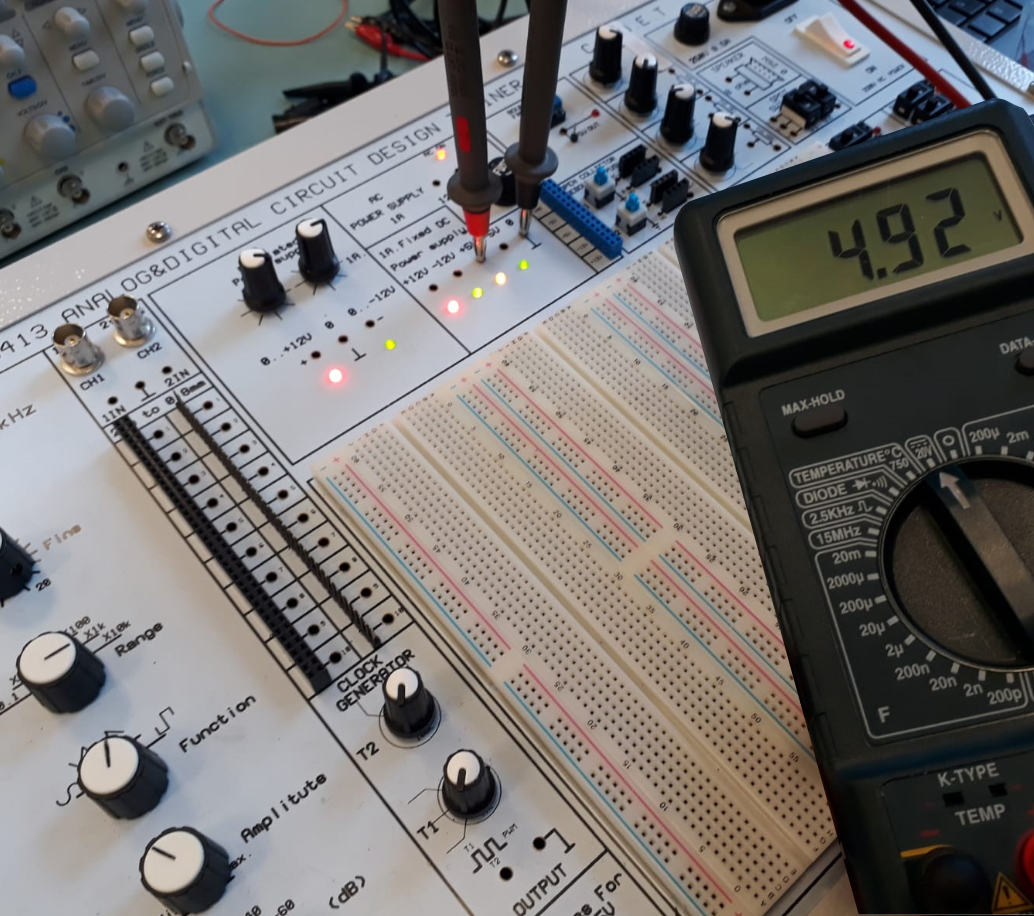
\includegraphics[width=0.5\textwidth]{6.jpg}
	\caption
	\label{Figure 6}
\end{figure}

Figure 6 shows that the potential difference we created was 4.92 volts

\begin{figure}[h]
	\centering
	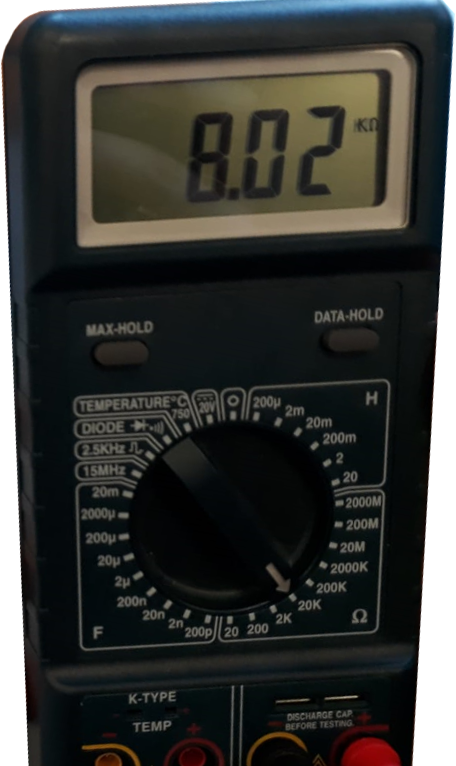
\includegraphics[height=0.5\textwidth]{7.jpg}
	\caption
	\label{Figure 7}
\end{figure}

In Figure 7 we can see that the resistance obtained was 8.02 Kohms.

\clearpage
\subsection{PART 4}
In this section we used 8 logic switches and 2 displays to show "27". 4 logic switches were used for each display.

\begin{figure}[h]
	\centering
	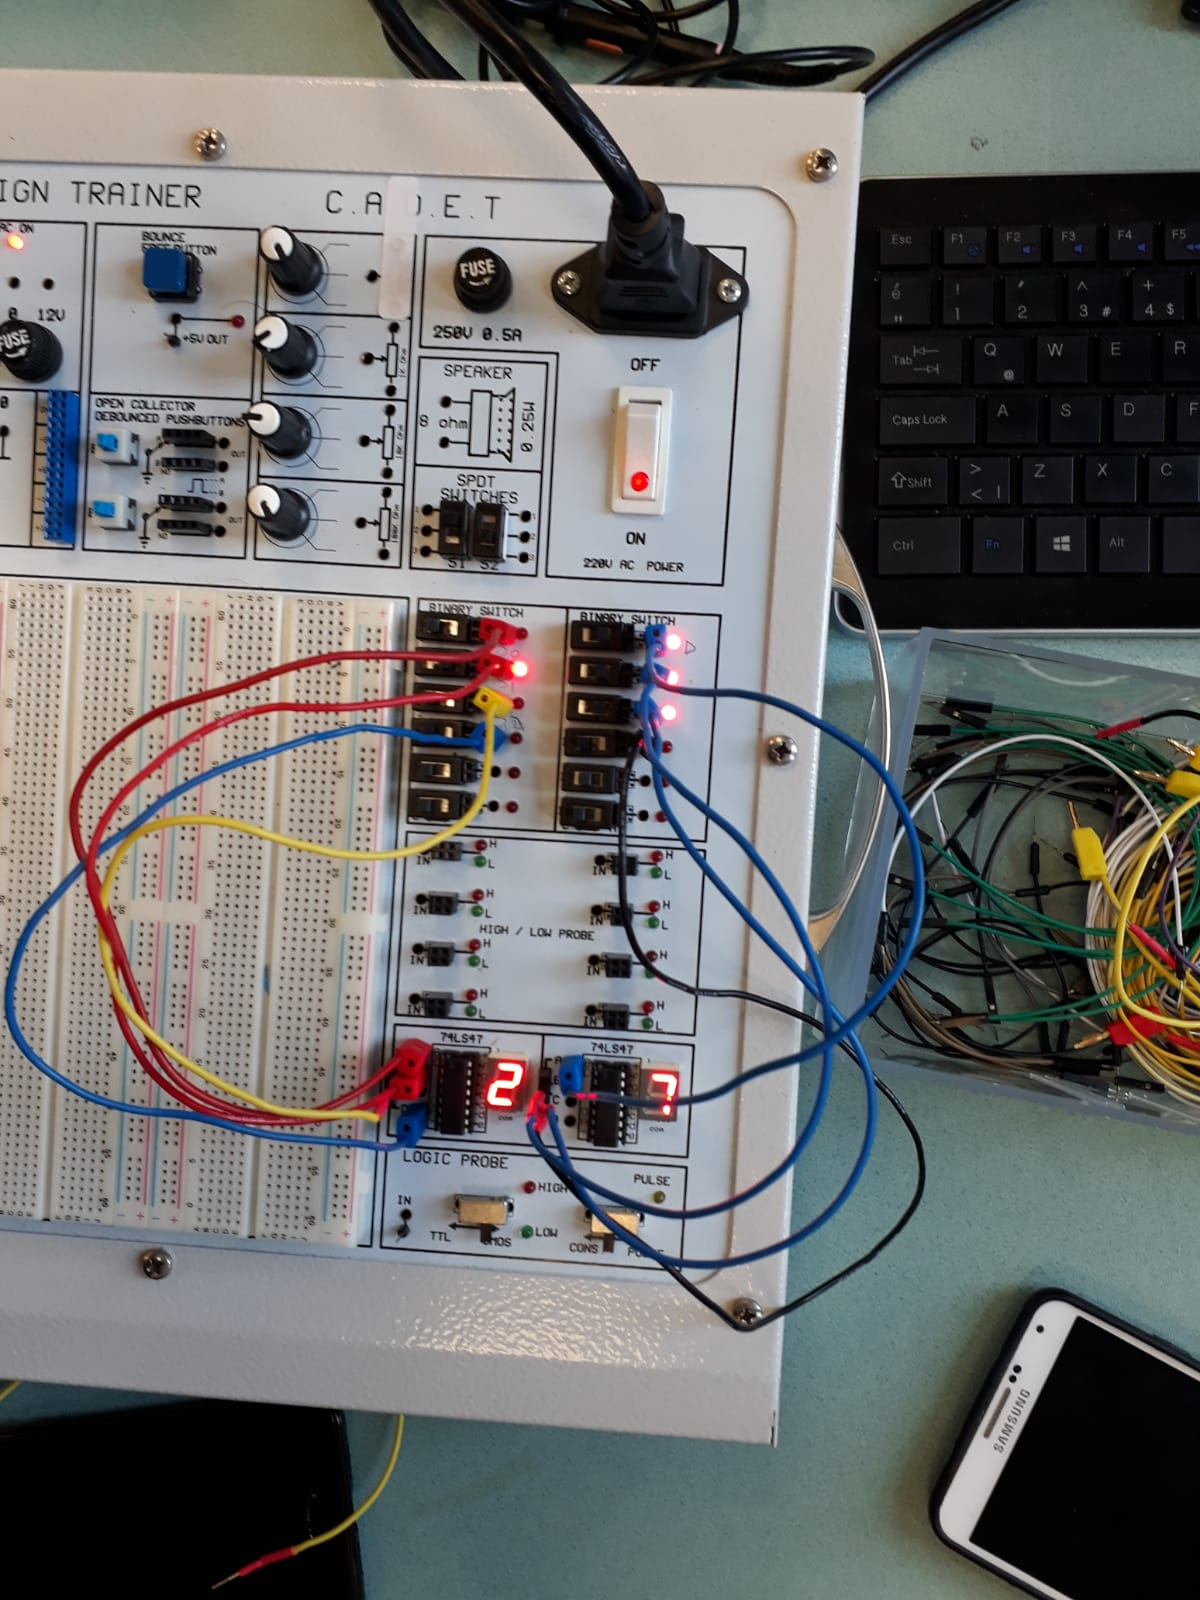
\includegraphics[width=0.5\textwidth]{8.jpg}
	\caption
	\label{Figure 8}
\end{figure}
From figure 8 it can be observed that the displays show the numbers "2" and "7" which were in binary form in displays inputs that were generated from the logic switches.

\begin{figure}[h]
	\centering
	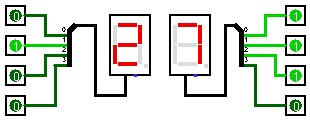
\includegraphics[width=0.5\textwidth]{8.1.jpg}
	\caption
	\label{Figure 8.1}
\end{figure}


\clearpage
\subsection{PART 5}
In this section of the experiment we used function generator to generate functions with different properties and used oscilloscope to observe the different functions 

\begin{figure}[h]
	\centering
	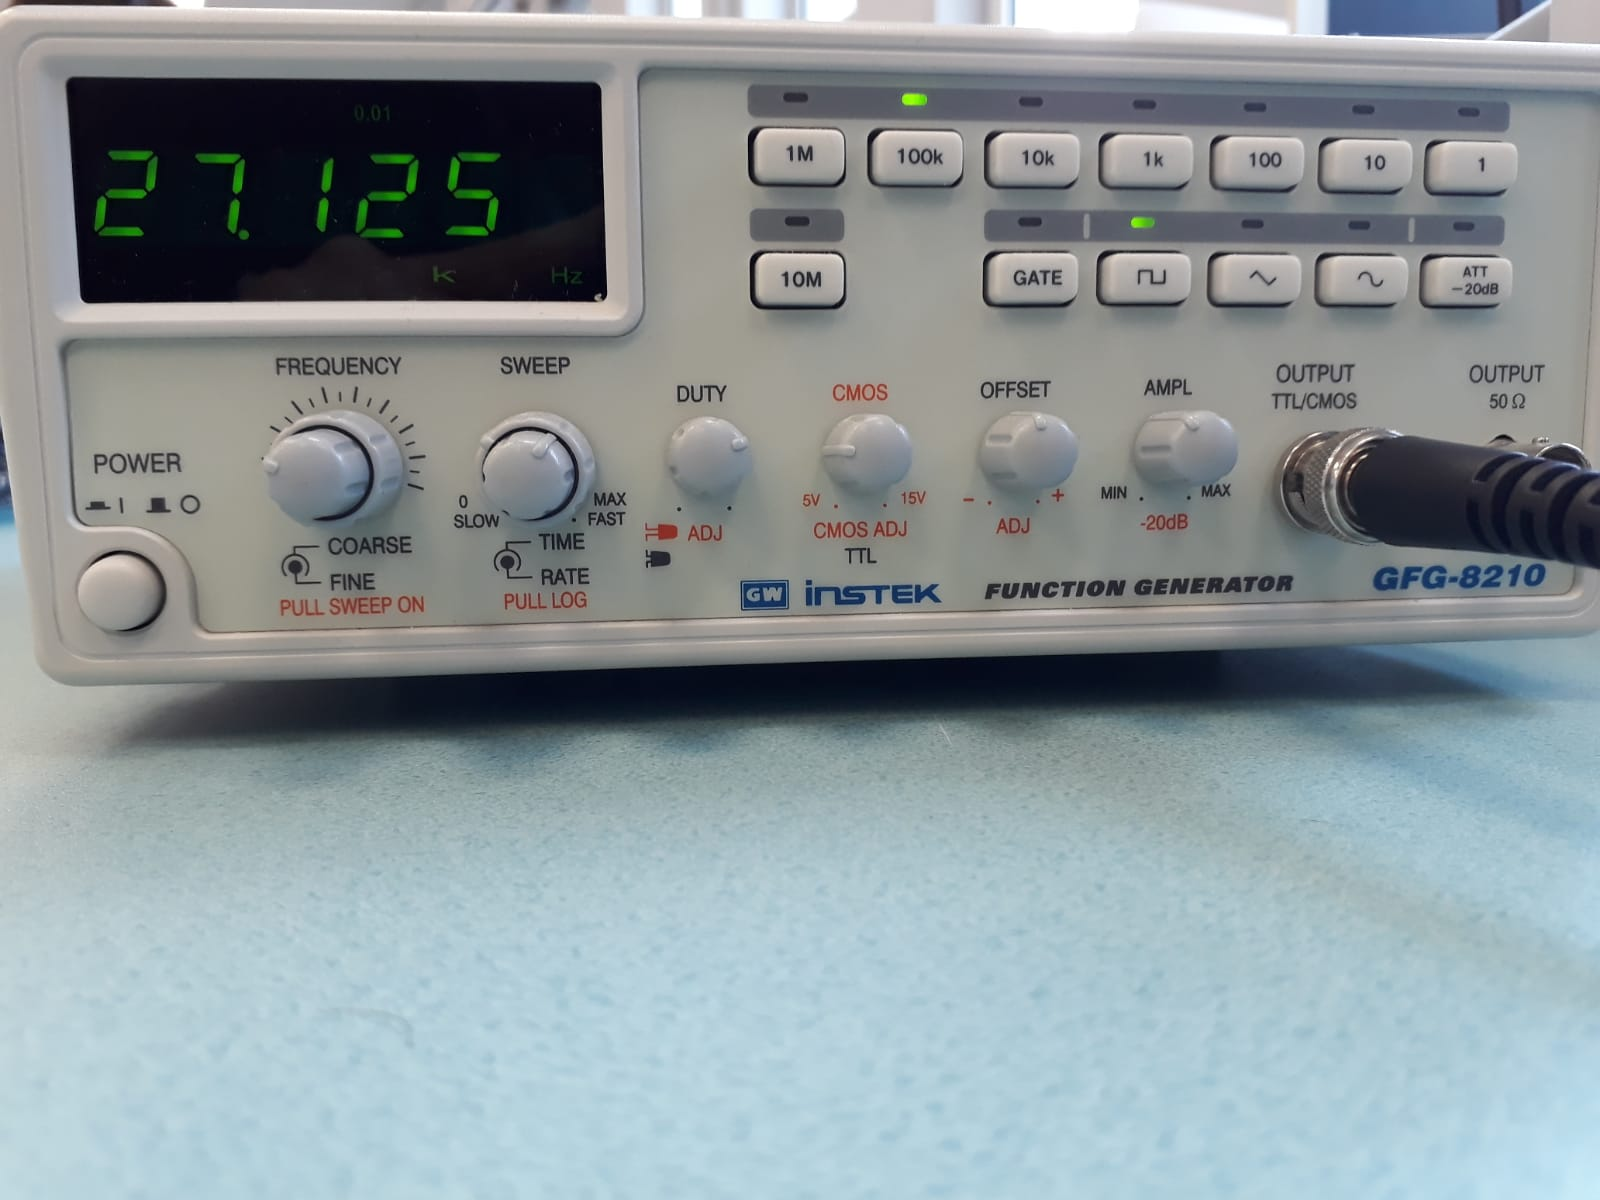
\includegraphics[width=0.5\textwidth]{9.jpg}
	\caption
	\label{Figure 9}
\end{figure}

\begin{figure}[h]
	\centering
	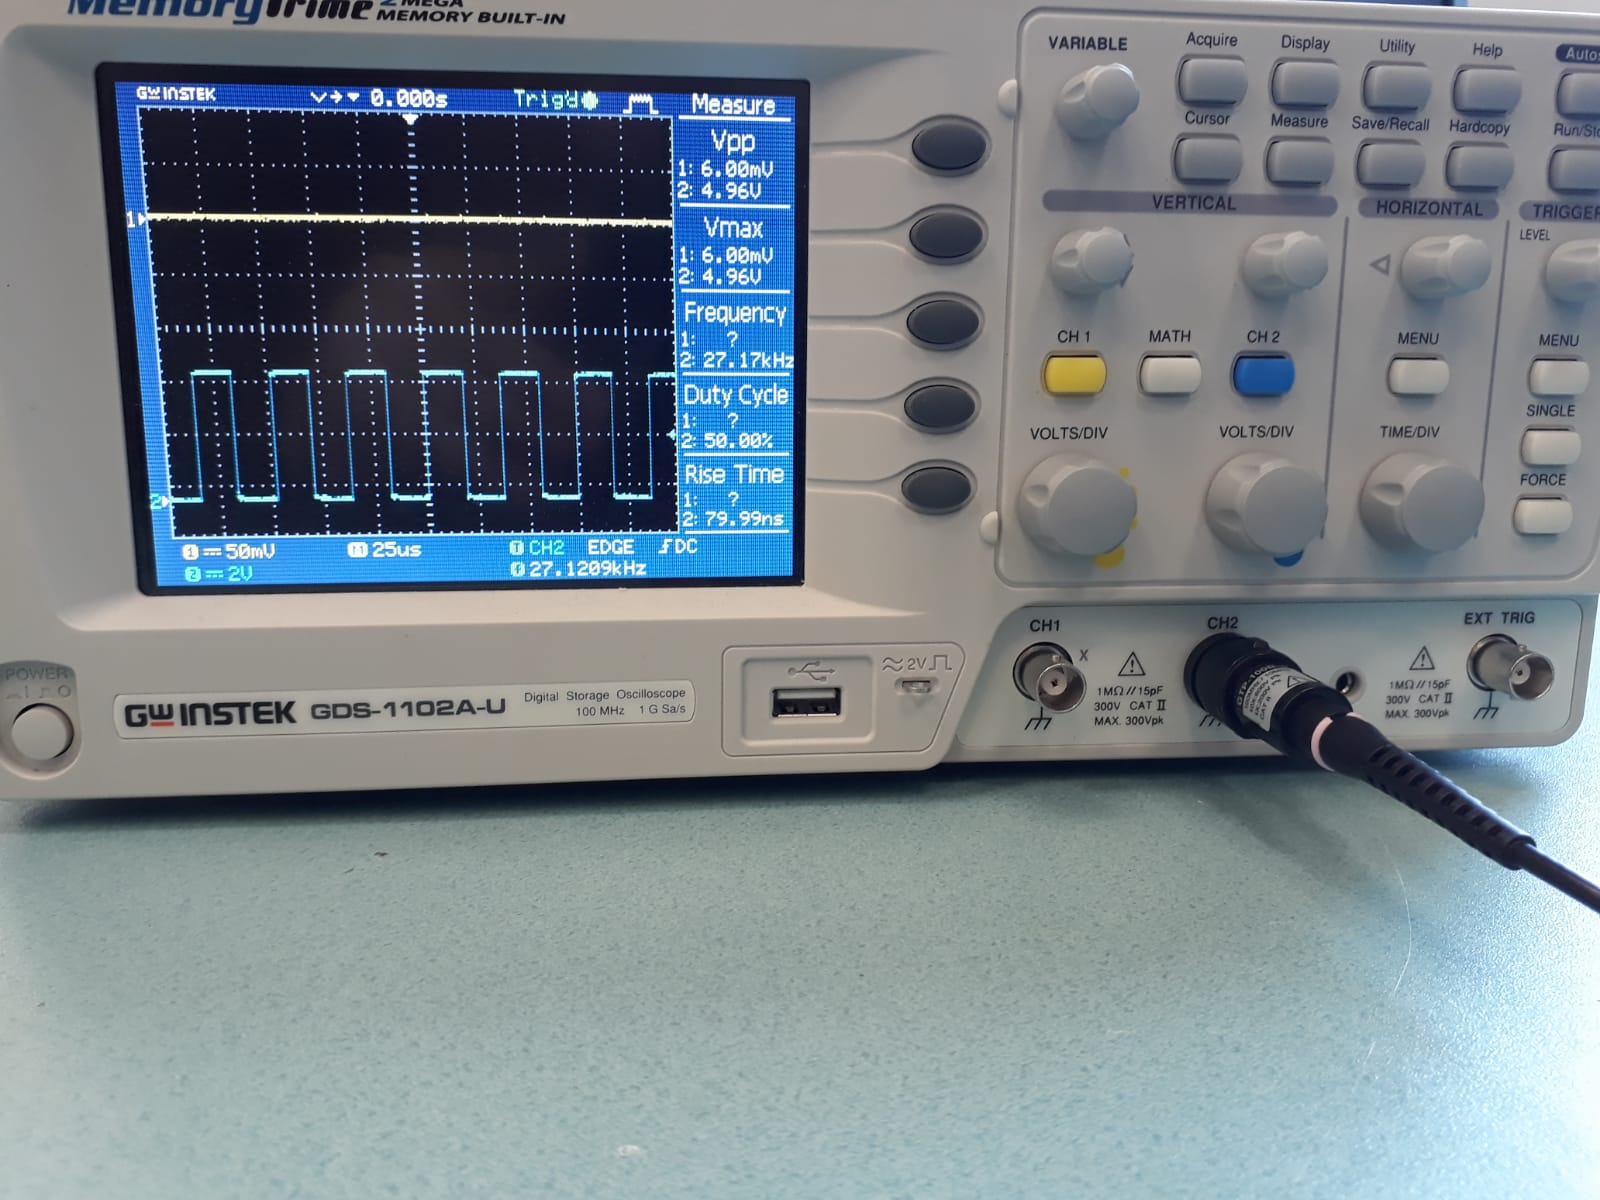
\includegraphics[width=0.5\textwidth]{10.jpg}
	\caption
	\label{Figure 10}
\end{figure}
From figure 9 and 10 we can see that the function generated and observed were approximately 27 kHz TTL wave.

\clearpage
\begin{figure}[h]
	\centering
	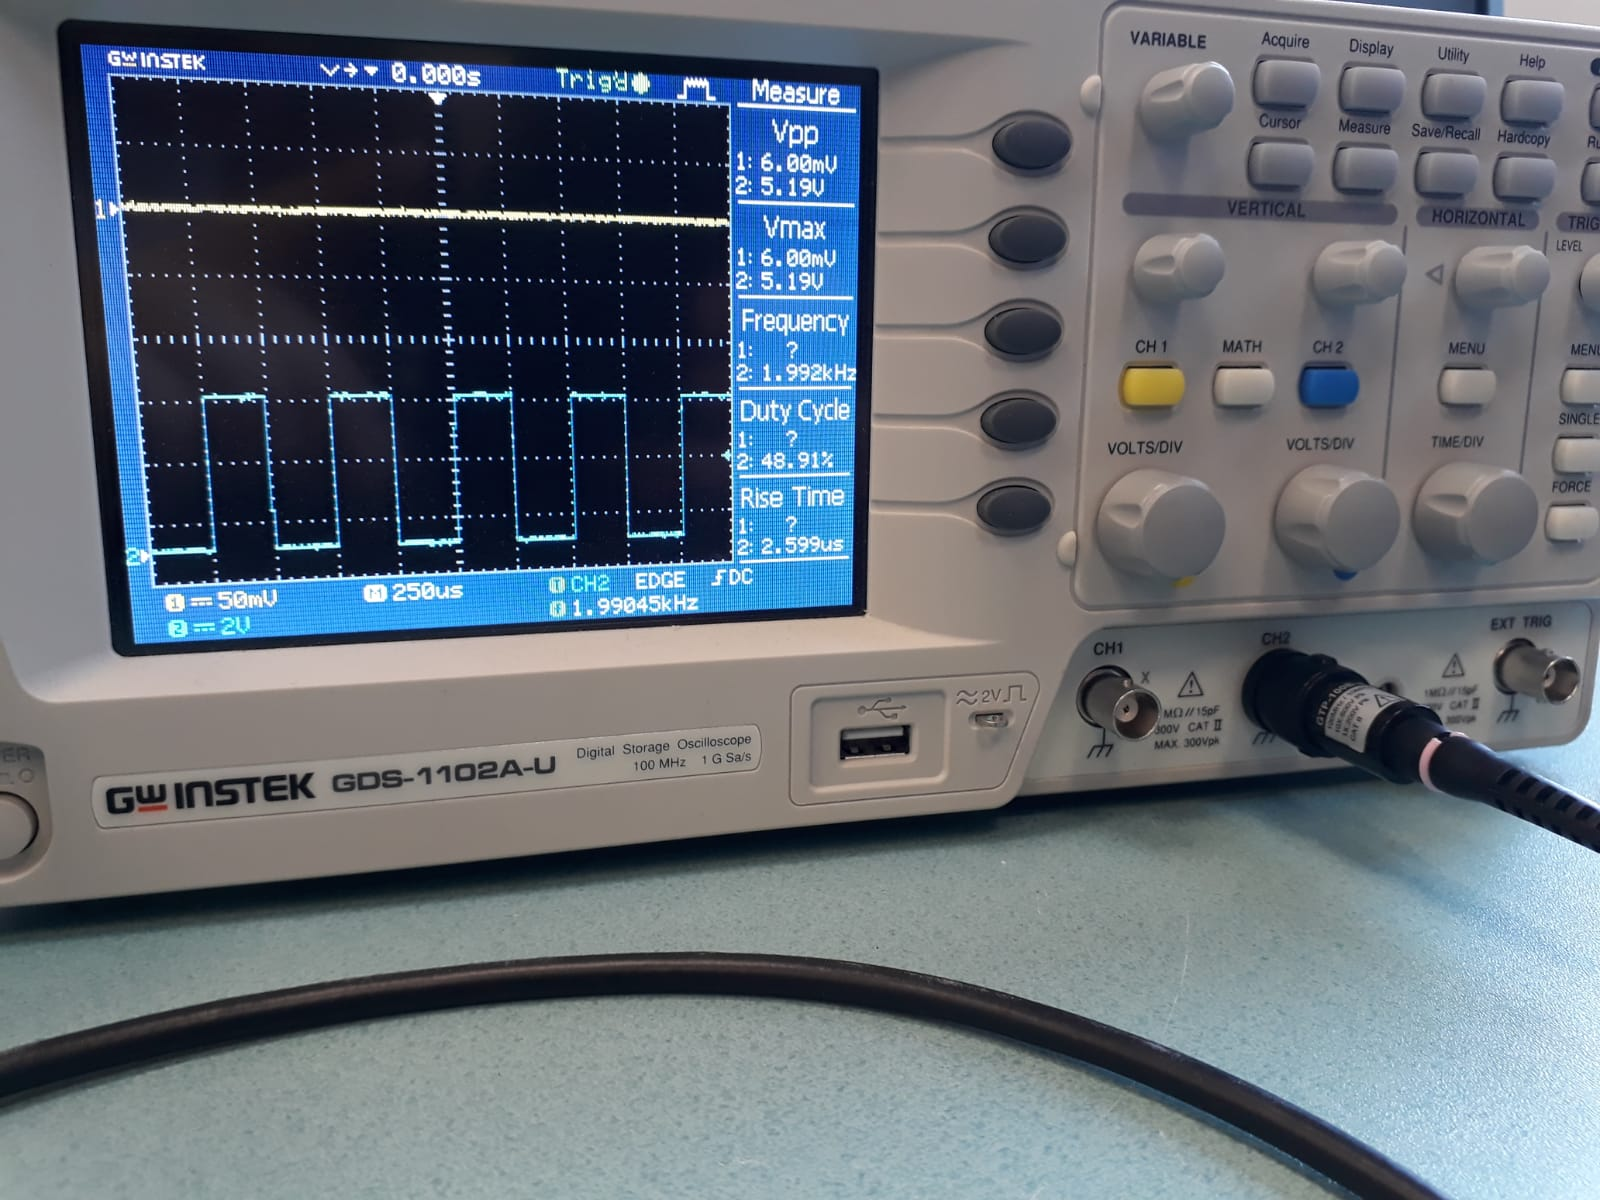
\includegraphics[width=0.5\textwidth]{11.jpg}
	\caption
	\label{Figure 11}
\end{figure}

\begin{figure}[h]
	\centering
	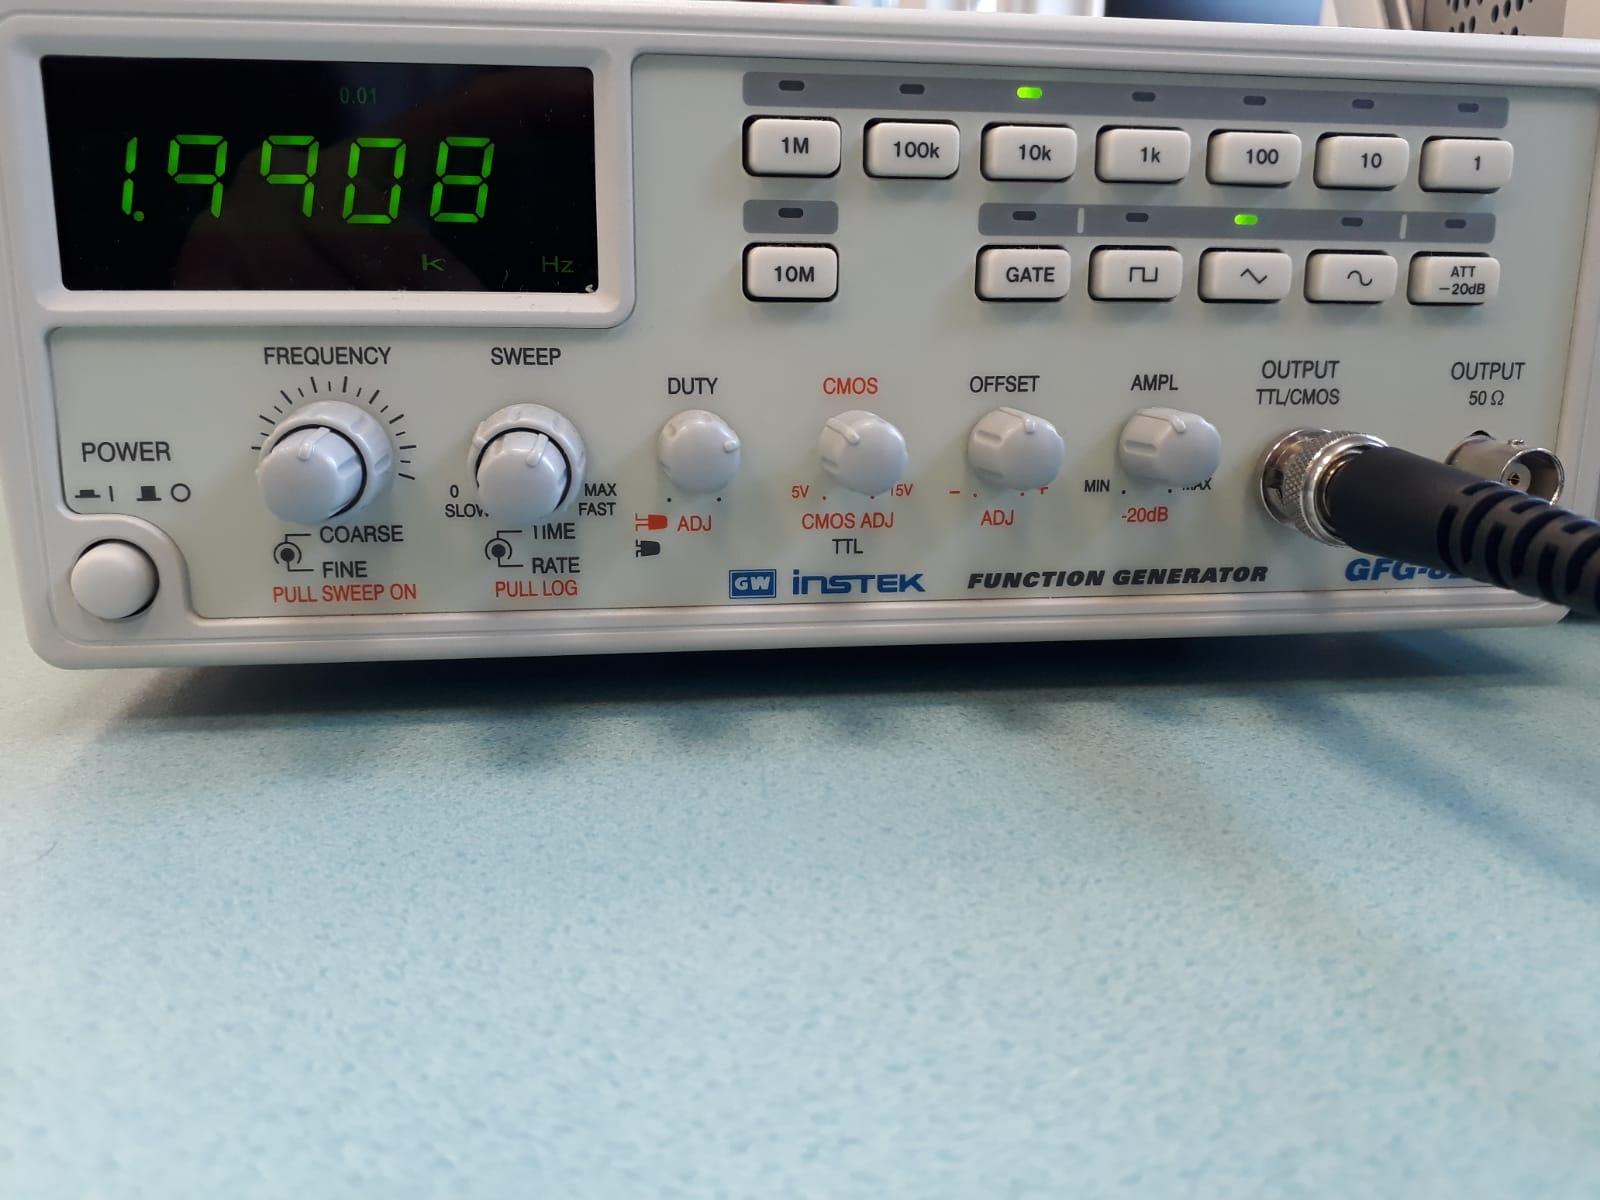
\includegraphics[width=0.5\textwidth]{12.jpg}
	\caption
	\label{Figure 12}
\end{figure}
From figure 11 and 12 it can observed that the function generated and observed were approximately 1992 Hz CMOS wave with Vpp of 5 Volts.

\clearpage
\section{RESULTS \& DISCUSSION}
The results we observed from the experiment were quite similar with the expected results, The errors in results were minimal and can be neglected. Since the part 2 and part 4 did not include voltage or resistance measurement or any type of function generation and observation, the results were certain and same with expected results. In part 5, we used function generator and the results we got from our observation was similar but not the same with the expected which could be based on sensitivity of the generator and measurement tool.


\section{CONCLUSION}
First four parts of the experiment was quite easy to complete since we were using basic components and certain measurements. Unlike the first four parts, other parts were challenging a bit since we were not familiar with the function generator.
\newline
\newline Things we learned from the experiment 1:
\begin{itemize}
    \item   Components of CADET.
    \item   How to use function generator and oscilloscope.
    \item   Difference between SPDT switch and logic switch.
    \item   Difference between TTL and CMOS(wave forms and voltage values).
    \item   Internal Structure of the 74x04 integrated circuit.
\end{itemize}

\newpage
\nocite{*}
\addcontentsline{toc}{section}{\numberline {}REFERENCES}

\bibliographystyle{unsrt}
\bibliography{reference}

\newpage
\addtocontents{toc}{\contentsline {section}{\numberline {}ETHICS}{}}

\thispagestyle{empty}
\centering{\LARGE{ \textbf{ETHIC FORM}}}\\
\centering{\LARGE{\textbf{for}}}\\
\centering{\LARGE{\textbf{BLG242E Logic Circuits Laboratory}}}\\[0.2cm]
As a student of \\Istanbul Technical University Faculty of Computer and Informatics Engineering;
\begin{enumerate}
    \item I will not attempt to cheat in quizes and final exam,
    \item I will not use disallowed sources or tools (mobile phone, calculator etc.) during the exam,
    \item I will not write any information (formula, text, figure etc.) on the table, sheets or books that are allowed to be used during the exam,
    \item I will give reference when using printed or online published sources,
    \item I will not use the results in a source as they are, or by changing a part of them without giving a reference,
    \item I will not show unused sources as used, 
    \item I will not present someone else’s idea as my own idea, 
    \item I will not make someone do my homework, project or thesis for money or anything else,
    \item I will not take an exam or enter a lecture on behalf of others,
    \item I will not make excuses for not attending in exams or lessons by taking reports from someone I know (medical doctor parents or relatives),
    \item I will refrain from deliberately harming the public materials at our university,  
    \item I will comply with the safety rules in laboratory work,
    \item I will behave in accordance with the rules of respect for the lecturers and teaching assistants
\end{enumerate}
\vspace{-1em}
\centering{\LARGE{signed by}}\\
\vspace{-1em}
\begin{table}[ht]
\centering
\begin{tabular}{rcl}
150160000  & : & STUDENT NAME \& SURNAME \\
150160001  & : & STUDENT NAME \& SURNAME \\
150160002  & : & STUDENT NAME \& SURNAME \\
\end{tabular}
\end{table}
\vspace{-1em}
 \begin{table}[ht]
 \begin{tabular}{lr}
\textbf{Date:\hspace*{1.0cm}/\hspace*{1.0cm}/} &\qquad \qquad\qquad\qquad \qquad\qquad\qquad \qquad\qquad\qquad \qquad\qquad \textbf{SIGNED}\\
\end{tabular}
\end{table}

\end{document}

